%%%%%%%%%%%%%%%%%%%%%%%%%%%%%%%%%%%%%%%%%%%%%%%%%%%%%%%%%%
%% 
%% MARK: Title
%%
%%%%%%%%%%%%%%%%%%%%%%%%%%%%%%%%%%%%%%%%%%%%%%%%%%%%%%%%%%

\addtocontents{toc}{\SkipTocEntry}
\chapter*{\S B8. Non-Symplectic Manifold with \\ Injective Universal Moment Map}
\addcontentsline{toc}{chapter}{\S B8. Non-symplectic manifold with injective univ. moment map}
\chaptermark{\S B8. Non-symplectic manifold with injective\dots}
\setcounter{footnote}{0}

%%%%%%%%%%%%%%%%%%%%%%%%%%%%%%%%%%%%%%%%%%%%%%%%%%%%%%%%%%
%% 
%% MARK: Abstract
%% 
%%%%%%%%%%%%%%%%%%%%%%%%%%%%%%%%%%%%%%%%%%%%%%%%%%%%%%%%%%

\begin{abstract}
  This addendum is an exercise,
  with a detailed solution,
  based on Note 2 of article 9.23 of the textbook.
  This example shows how the condition of transitivity of the automorphisms is necessary for being a symplectic manifold.
\end{abstract}

Considering the program of symplectic diffeology,
I have suggested calling a symplectic differential form on a diffeological space $X$ any closed $2$-form $\omega$ satisfying the following two properties:

\begin{enumerate}
  \item The universal moment map $\mu_\omega : X \to  \cG_\omega$ is injective.
  \item The local automorphisms $\Diff_\loc(X,\omega)$ are transitive on $X$.
\end{enumerate}

The first condition is to avoid non-zero characteristics of $\omega$ because of the theorem \cite[\textsection\,9.26]{PIZ13} claiming that for manifolds homogeneous under $\Diff(X,\omega)$,
the characteristics of $\omega$ are precisely the pre-images of the universal moment map.

The second condition is the transposition to diffeology of the Darboux theorem satisfied by symplectic manifolds.
It could be strengthened by considering the group of automorphisms,
which is still satisfied for manifolds,
but it does not seem necessary to do so.

Now,
we shall see why the second condition is necessary by constructing an example of a closed $2$-form on a manifold for which the universal moment map is injective but the group of automorphisms is not transitive.

\begin{Article}{Exercise.}{}
  \label{Injective-universal-moment-map-for-a-non-symplectic-form} 
  Let us consider the real plane $\RR^2$ equipped with the $2$-form
  $$
    \omega = (x^2 + y^2)\, dx \wedge dy.
    $$
  \Question{\bf Q1.} Why is $\omega$ closed?
  \Question{\bf Q2.} Describe the kernel of $\omega$.
  Assuming that the group of
  compactly supported automorphisms of a symplectic manifold is transitive,
  deduce that $\Diff(\RR^2, \omega)$,
  the group of automorphisms of $\omega$,
   has two orbits:
  $\{0_{\RR^2}\}$ and $\RR^2 - \{0_{\RR^2}\}$.
  \Question{\bf Q3.} Explain why every automorphism of $(\RR^2, \omega)$ is Hamiltonian.
  \Question{\bf Q4.} Exhibit the unique equivariant universal moment map $\mu_\omega$
  for $(\RR^2, \omega)$ such that $\mu_\omega(0_{\RR^2}) = 0_{\cG^*}$.
   Why is it unique?
  \Question{\bf Q5.} Show that if $z=(x,y) \neq (0,0)$,
  then $\mu_\omega(z) \neq 0_{\cG^*}$.
  Conclude that $\mu_\omega$ is injective.
\end{Article}

\begin{proof}
  Q1. $\omega$ is closed because it is a $2$-form on a $2$-dimensional space (op.\,cit. \textsection\,6.39).
  
  Q2. Let $z = (x,y) \in \RR^2$.
  By definition,
  $$
    \ker(\omega_z) = \{u \in \RR^2 \mid \omega_z(u)(v) = 0 \mbox{ for all } v \in \RR^2 \}.
    $$
  But $\omega_z(u)(v) = (x^2 + y^2) \det(u\, v)$.
  Thus,
   since $\det( \cdot\, \cdot )$ is nondegenerate,
  if $z \neq (0,0)$ then $\ker(\omega_z) = \{0_{\RR^2}\}$,
  whereas $\ker(\omega_0) = \RR^2$.
  
  Since an automorphism of $\omega$ induces an isomorphism on the kernel,
  the origin $0_{\RR^2}$ must be mapped to itself by any automorphism of $\omega$.
  Indeed,
  $0_{\RR^2}$ is the only point with kernel $\RR^2$.
  Then,
  for all $\varphi \in \Diff(\RR^2,\omega)$,
  $\RR^2-\{0\}$ is invariant under $\varphi$,
  so $\varphi \restriction \RR^2-\{0_{\RR^2}\}$ is a symplectomorphism of $\RR^2-\{0_{\RR^2}\}$.
  Now,
   $\RR^2-\{0_{\RR^2}\}$ is open and $\omega \restriction \RR^2-\{0_{\RR^2}\}$ is symplectic.
   By the assumption:
  for every two points $z$ and $z'$ in $\RR^2-\{0_{\RR^2}\}$ there exists a compactly supported automorphism $\varphi$ of $(\RR^2-\{0_{\RR^2}\}, \omega \restriction \RR^2-\{0_{\RR^2}\})$ mapping $z$ to $z'$.
  But since a compact set in $\RR^2-\{0_{\RR^2}\}$ is closed and bounded,
  the complement of the support contains an open neighborhood of $0_{\RR^2}$ on which $\varphi$ is the identity;
  thus $\varphi$ can be smoothly extended by setting $\varphi(0_{\RR^2}) = 0_{\RR^2}$.
  This extension,
  still mapping $z$ to $z'$,
  clearly satisfies $\varphi^*(\omega) = \omega$ on $\RR^2$ and then belongs to $\Diff(\RR^2,\omega)$.
  Therefore,
  $\Diff(\RR^2,\omega)$ is transitive on $\RR^2 - \{0\}$;
  that is,
  the group $\Diff(\RR^2,\omega)$ has two orbits in $\RR^2$: $\{0_{\RR^2}\}$ and $\RR^2 - \{0_{\RR^2}\}$.
  
  Q3. Since $\RR^2$ is contractible (more precisely, has vanishing first homology),
  the automorphisms in $\Diff(\RR^2,\omega)$ are Hamiltonian (op.\,cit. \textsection\,9.7 and 9.15).
  
  Q4. Because the action of $\Diff(\RR^2,\omega)$ has a fixed point,
  $0_{\RR^2}$,
  the moment map is exact and there exists an invariant primitive $\mu_\omega$ (op.\,cit. \textsection\,9.10, Note 2).
  Applying the expressions $(\diamondsuit)$ and $(\heartsuit)$ of (op.\,cit. \textsection\,9.20) to a path $p$ connecting $0_{\RR^2}$ to $z=(x,y)$,
  an equivariant primitive $\mu_\omega$ (op.\,cit. \textsection\,9.9) of the $2$-point moment map (op.\,cit. \textsection\,9.8) is given,
   for every plot $F$ of $\Diff(\RR^2,\omega)$,
   by
  $$
    \mu_\omega(z)(F)_r(\delta r) = \int_0^1\omega_{p(t)}(\dot p(t))(\delta p(t))\, dt, 
    $$
  with
  $$
    \delta p(t) = [\Der(F(r))(p(t))]^{-1} {\partial F(r)(p(t)) \over \partial r} (\delta r).
    $$
  This moment map is unique because two moment maps differ only by a constant in $\cG^*$
  (since $\RR^2$ is connected) (op.\,cit. \textsection\,9.9),
  and the constant is fixed by the condition $\mu_\omega(0_{\RR^2}) = 0_{\cG^*}$.
  
  Q5. The proof that the moment map $\mu_\omega$,
   restricted to $\RR^2 - \{0_{\RR^2}\}$,
    is injective is contained in the proof of (op.\,cit. \textsection\,9.23, B) by choosing a real smooth function $f$ on $\RR^2$ vanishing outside a small ball centered at $z' \neq z$ not containing $z$ nor $0_{\RR^2}$.
    Now we just need to show that for all $z \in \RR^2 - \{0_{\RR^2}\}$, $\mu_\omega(z) \neq 0_{\cG^*}$.
  For that we apply the previous formula to
  $$
    p(t) = tz \SpacedText{and} F(r) =
    \begin{pmatrix} 
    \cos(2\pi r) & -\sin(2\pi r) \\
    \sin(2\pi r) & \cos(2\pi r) 
    \end{pmatrix},
    $$
  with
  $$
    t \in \RR, \quad z=(x,y)  \in \RR^2, \quad r \in \RR \SpacedText{and} \delta r = 1.
    $$
  By linearity, $\Der(F(r))(p(t)) = F(r)$,    
  and then
  %
  \begin{multline*}
    \delta p(t) = F(r)^{-1}{\partial F(r) \over \partial r} (p(t)) \\
    =
    \begin{pmatrix} 
      \cos(2\pi r) & \sin(2\pi r) \\
      -\sin(2\pi r) & \cos(2\pi r) 
    \end{pmatrix}
    \times 2\pi \times 
    \begin{pmatrix} 
      -\sin(2\pi r) & -\cos(2\pi r) \\
      \cos(2\pi r) & -\sin(2\pi r) 
    \end{pmatrix}
    \begin{pmatrix} 
      tx \\
      ty
    \end{pmatrix}\\
    =
    2\pi
    \begin{pmatrix} 
      0 & -1 \\
      1 & 0 
    \end{pmatrix}
    \begin{pmatrix} 
      tx \\
      ty
    \end{pmatrix}
    =
    2\pi
    \begin{pmatrix} 
      -ty \\
      tx
    \end{pmatrix}.
  \end{multline*}
  %
  On the other hand,
  $\dot p(t) = {d(tz) \over dt} = z$.
  Hence,
  $$
    \dot p(t) = \begin{pmatrix} 
    x \\
    y
    \end{pmatrix}, 
    \SpacedText{and}
    \delta p(t) = 2\pi
    \begin{pmatrix} 
    -ty \\
    tx
    \end{pmatrix}.
    $$
  Therefore,
  %
  \begin{multline*}
    \mu_\omega(z)(F)_r(\delta r)
    =
    \int_0^1\omega_{p(t)}(\dot p(t))(\delta p(t)) dt
    = 2\pi \int_0^1\omega_{tz}
    \begin{pmatrix} 
      x \\
      y
    \end{pmatrix}
    \begin{pmatrix}
      -ty \\
      tx
    \end{pmatrix}
     dt
    \\
    =
   2\pi \int_0^1 ((tx)^2 + (ty)^2) \det
    \begin{pmatrix} 
      x & -y \\
      y & x 
    \end{pmatrix}  t dt
    \\
    =  2\pi \int_0^1 (x^2 + y^2)^2 t^3  dt
    = 2\pi (x^2 + y^2)^2 \int_0^1  t^3 \, dt
    = \frac{2\pi}{4} (x^2 + y^2)^2.
  \end{multline*}
  %
  Hence,
  if $z=(x,y) \neq (0,0)$,
  the value of the moment map above,
  computed on the $1$-parameter family $F$,
  is non-zero,
   which implies $\mu_\omega(z) \neq 0_{\cG^*}$.
  
  In conclusion, $\mu_\omega(0_{\RR^2}) = 0_{\cG^*}$, 
  $\mu_\omega \restriction \RR^2 - \{0_{\RR^2}\}$ is injective,
  and if $z \neq 0_{\RR^2}$ then $\mu_\omega(z) \neq  0_{\cG^*}$;
  therefore $\mu_\omega$ is injective.
\end{proof}

\bigskip
\uline{So, what is this exercise all about?} Paragraph 9.23 states that a closed
$2$-form $\omega$ on a manifold is symplectic,
that is,
nondegenerate,
if and only if its group of automorphisms is transitive and the universal moment map is injective.
This exercise shows that the injectivity of the universal moment map alone is not sufficient
(the condition of transitivity is necessary), 
since it exhibits a non-symplectic closed $2$-form on $\RR^2$ with an injective universal moment map.

%\vfill\n
%\centerline{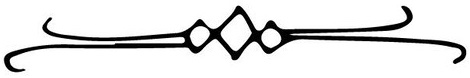
\includegraphics[width=.5\textwidth]{Figures/separator.jpg}}\n
